\documentclass[11pt,a4paper]{article}

% ─── Packages ───────────────────────────────────────────────────────────────
\usepackage[T1]{fontenc}
\usepackage[utf8]{inputenc}
\usepackage[margin=2.5cm]{geometry}
\usepackage{amsmath,amssymb}
\usepackage{booktabs}
\usepackage{graphicx}
\usepackage{hyperref}
\usepackage{xcolor}
\usepackage{caption}
\usepackage{subcaption}
\usepackage{parskip}
\usepackage{enumitem}
\usepackage{float}
\usepackage{url}
\usepackage{algorithm}
\usepackage{algpseudocode}
\usepackage{array}
\usepackage{multirow}
\usepackage{siunitx}

\hypersetup{
    colorlinks=true,
    linkcolor=blue!60!black,
    citecolor=blue!60!black,
    urlcolor=blue!60!black
}

% ─── Title ──────────────────────────────────────────────────────────────────
\title{\textbf{An Experimental Comparison of Sorting Algorithms}\\[0.4em]
\large MPI(L)2026 — Methods of Programming Investigation}

\author{%
  Umar Sabir\\
  \small West University of Timi\c{s}oara\\
  \small \texttt{umar.sabir11@e-uvt.ro}
}

\date{May 2026}

% ─── Document ───────────────────────────────────────────────────────────────
\begin{document}

\maketitle

\begin{abstract}
Sorting is a fundamental computational problem with a rich landscape of algorithmic
solutions, each with distinct theoretical complexities and practical behaviours.
This paper presents a systematic experimental comparison of ten sorting algorithms:
\emph{Bubble Sort}, \emph{Selection Sort}, \emph{Insertion Sort}, \emph{Shell Sort},
\emph{Merge Sort}, \emph{Quick Sort} (median-of-three pivot), \emph{Heap Sort},
\emph{Counting Sort}, \emph{Radix Sort}, and \emph{Tim Sort}.
We measure average running time over five independent trials across four input
distributions (random, already-sorted, reverse-sorted, and nearly-sorted) and six
input sizes ($n \in \{100, 500, 1000, 2000, 5000, 10000\}$).
Our results confirm well-known theoretical predictions while exposing non-obvious
practical trade-offs: Quick Sort with median-of-three consistently outperforms Merge
Sort by a constant factor on random data; Counting and Radix Sort achieve near-linear
empirical growth; and Insertion Sort surpasses all $\mathcal{O}(n\log n)$ algorithms
on nearly-sorted input of moderate size.
All source code and raw results are available at
\url{https://github.com/umarkhattak256-sketch/sorting-algorithms-experiment}.
\end{abstract}

\tableofcontents
\newpage

% ────────────────────────────────────────────────────────────────────────────
\section{Introduction}
% ────────────────────────────────────────────────────────────────────────────

Sorting is arguably the most studied algorithmic problem in computer science.
It underpins database query processing, search engine indexing, compiler symbol-table
management, and a wide range of combinatorial algorithms that require pre-sorted input.
Despite decades of research, no single algorithm dominates all scenarios: the choice
depends on input size, input distribution, memory constraints, hardware cache
behaviour, and implementation language.

The primary contribution of this paper is \emph{empirical}: we measure wall-clock time
rather than operation counts, observe how theory translates (or fails to translate)
into practice, and highlight conditions under which commonly-taught algorithms
are outperformed by simpler alternatives.

\paragraph{Research questions.}
\begin{enumerate}[label=RQ\arabic*.]
  \item Do empirical growth rates match theoretical complexity classes?
  \item How sensitive is each algorithm to the initial ordering of the input?
  \item Under what conditions do $\mathcal{O}(n^2)$ algorithms remain competitive?
  \item Do linear-time non-comparison sorts provide measurable advantages at the
        sizes we test?
\end{enumerate}

The remainder of this paper is organised as follows.
Section~\ref{sec:background} reviews the algorithms and their complexities.
Section~\ref{sec:methodology} describes the experimental setup.
Section~\ref{sec:results} presents and discusses the results.
Section~\ref{sec:threats} addresses threats to validity.
Section~\ref{sec:conclusion} concludes.

% ────────────────────────────────────────────────────────────────────────────
\section{Background and Algorithm Descriptions}
\label{sec:background}
% ────────────────────────────────────────────────────────────────────────────

Table~\ref{tab:complexity} summarises the theoretical time and space complexities of
all ten algorithms.

\begin{table}[H]
\centering
\caption{Theoretical complexity of the ten sorting algorithms studied.
  $n$ = input size; $k$ = value range for Counting/Radix Sort;
  $d$ = number of digits for Radix Sort.}
\label{tab:complexity}
\small
\renewcommand{\arraystretch}{1.25}
\begin{tabular}{@{}lcccc@{}}
\toprule
\textbf{Algorithm} & \textbf{Best case} & \textbf{Average case} & \textbf{Worst case} & \textbf{Space} \\
\midrule
Bubble Sort    & $\Omega(n)$           & $\Theta(n^2)$          & $\mathcal{O}(n^2)$    & $\mathcal{O}(1)$ \\
Selection Sort & $\Theta(n^2)$         & $\Theta(n^2)$          & $\mathcal{O}(n^2)$    & $\mathcal{O}(1)$ \\
Insertion Sort & $\Omega(n)$           & $\Theta(n^2)$          & $\mathcal{O}(n^2)$    & $\mathcal{O}(1)$ \\
Shell Sort     & $\Omega(n\log n)$     & $\Theta(n^{4/3})$      & $\mathcal{O}(n^{3/2})$& $\mathcal{O}(1)$ \\
Merge Sort     & $\Theta(n\log n)$     & $\Theta(n\log n)$      & $\Theta(n\log n)$     & $\mathcal{O}(n)$ \\
Quick Sort     & $\Omega(n\log n)$     & $\Theta(n\log n)$      & $\mathcal{O}(n^2)$    & $\mathcal{O}(\log n)$ \\
Heap Sort      & $\Theta(n\log n)$     & $\Theta(n\log n)$      & $\Theta(n\log n)$     & $\mathcal{O}(1)$ \\
Counting Sort  & $\Theta(n+k)$         & $\Theta(n+k)$          & $\Theta(n+k)$         & $\mathcal{O}(k)$ \\
Radix Sort     & $\Theta(dn)$          & $\Theta(dn)$           & $\Theta(dn)$          & $\mathcal{O}(n+k)$ \\
Tim Sort       & $\Omega(n)$           & $\Theta(n\log n)$      & $\mathcal{O}(n\log n)$& $\mathcal{O}(n)$ \\
\bottomrule
\end{tabular}
\end{table}

\subsection{Quadratic Algorithms}

\paragraph{Bubble Sort.}
Bubble Sort iterates through the array, repeatedly swapping adjacent elements that are
out of order. Each full pass ``bubbles'' the largest unsorted element to its correct
position. An early-termination flag makes it $\mathcal{O}(n)$ on already-sorted input.
Its $\mathcal{O}(n^2)$ average behaviour and high constant factor make it impractical
for large inputs, though its simplicity makes it pedagogically valuable.

\paragraph{Selection Sort.}
Selection Sort divides the array into a sorted prefix and an unsorted suffix.
On each pass it selects the minimum of the suffix and appends it to the sorted prefix.
Unlike Bubble Sort, it performs at most $n-1$ swaps, which can be advantageous when
write operations are expensive. Its running time is $\Theta(n^2)$ regardless of input
distribution.

\paragraph{Insertion Sort.}
Insertion Sort maintains a sorted prefix and inserts each new element into its correct
position within that prefix by shifting larger elements rightward.
It achieves $\mathcal{O}(n + I)$ time where $I$ is the number of inversions in the
input, making it extremely fast on nearly-sorted data and optimal for very small arrays.
Tim Sort exploits this property internally.

\subsection{Sub-quadratic Algorithms}

\paragraph{Shell Sort.}
Shell Sort generalises Insertion Sort by sorting elements separated by a gap $h$,
reducing the gap sequence until $h = 1$ (at which point it degenerates to Insertion
Sort). We use the Knuth gap sequence $h_k = (3^k - 1)/2$.
The analysis of Shell Sort is notoriously difficult; empirically it behaves near
$\mathcal{O}(n^{1.25})$ in practice.

\subsection{Optimal Comparison-Based Algorithms}

\paragraph{Merge Sort.}
Merge Sort divides the array in half, recursively sorts each half, and merges the two
sorted halves in linear time. It is a stable, deterministic $\Theta(n \log n)$ algorithm
but requires $\mathcal{O}(n)$ auxiliary space. Its stable comparison count is
approximately $n \log_2 n - n$.

\paragraph{Quick Sort.}
We implement Quick Sort with a \emph{median-of-three} pivot selection strategy,
choosing the median of the first, middle, and last elements. This avoids worst-case
$\mathcal{O}(n^2)$ performance on sorted and reverse-sorted inputs, which plague the
naive first-element pivot strategy. Quick Sort is in-place and has excellent cache
locality due to sequential memory access patterns, typically outperforming Merge Sort
in practice.

\paragraph{Heap Sort.}
Heap Sort builds a max-heap in $\mathcal{O}(n)$ time using Floyd's algorithm, then
repeatedly extracts the maximum element, yielding a sorted array. It is in-place and
guarantees $\Theta(n \log n)$ in all cases. However, its poor cache behaviour
(due to non-sequential memory access in the heap structure) makes it slower than Quick
Sort and Merge Sort in practice despite identical asymptotic complexity.

\paragraph{Tim Sort.}
Tim Sort is a hybrid algorithm combining Merge Sort and Insertion Sort, designed and
used as Python's built-in sort since Python 2.3. It identifies natural or synthetic
``runs'' (already-ordered subsequences) and merges them efficiently using a stack-based
merge strategy. It is particularly effective on real-world data, which frequently
contains partially-ordered subsequences.

\subsection{Linear-Time Non-Comparison Sorts}

\paragraph{Counting Sort.}
Counting Sort counts the occurrences of each distinct value and reconstructs the sorted
array from the counts. It runs in $\Theta(n + k)$ time and space, where $k$ is the
range of input values. In our benchmarks, $k = 10n$, so Counting Sort's space and
time usage scales slightly super-linearly with $n$.

\paragraph{Radix Sort.}
Radix Sort applies Counting Sort digit-by-digit from the least significant digit (LSD)
to the most significant digit, sorting stably at each pass. With base-10 and values
in $[0, 10n)$, the number of passes $d = \lceil \log_{10}(10n) \rceil = \lceil 1 + \log_{10}(n) \rceil$,
growing very slowly with $n$. This gives a practical $\mathcal{O}(n)$ behaviour for
the sizes we test.

% ────────────────────────────────────────────────────────────────────────────
\section{Methodology}
\label{sec:methodology}
% ────────────────────────────────────────────────────────────────────────────

\subsection{Implementation}

All algorithms are implemented in \textbf{Python 3.12} and are available at:
\begin{center}
\url{https://github.com/umarkhattak256-sketch/sorting-algorithms-experiment}
\end{center}
Each implementation operates on Python lists of integers and returns a new sorted list,
ensuring no in-place side effects affect timing of subsequent runs. Tim Sort invokes
Python's built-in \texttt{list.sort()}, which is implemented in C and serves as a
performance upper bound for what a production-grade implementation can achieve.

\subsection{Experimental Setup}

\paragraph{Hardware and software.}
Experiments were conducted on a machine running Ubuntu 24 LTS with Python 3.12.
Process affinity was not pinned; however, each measurement is the average of five
independent trials, mitigating transient OS scheduling noise.

\paragraph{Input sizes.}
We test $n \in \{100, 500, 1000, 2000, 5000, 10000\}$.
The $\mathcal{O}(n^2)$ algorithms (Bubble, Selection, Insertion Sort) are excluded from
sizes $n \geq 5000$ to keep benchmark time tractable.

\paragraph{Input distributions.}
\begin{itemize}[leftmargin=2em]
  \item \textbf{Random}: a random permutation of $n$ distinct values from $[0, 10n)$.
  \item \textbf{Sorted}: the sequence $[0, 1, \ldots, n-1]$.
  \item \textbf{Reverse-sorted}: the sequence $[n, n-1, \ldots, 1]$.
  \item \textbf{Nearly-sorted}: a sorted sequence with $\lfloor n/20 \rfloor$ random
        adjacent swaps applied.
\end{itemize}

\paragraph{Measurement.}
Each $(algorithm, input\_type, n)$ combination is executed $r = 5$ independent times.
Wall-clock time is measured using Python's \texttt{time.perf\_counter()}, which
provides sub-microsecond resolution. The arithmetic mean of the five measurements is
reported. Input generation time is excluded from measurements.

\paragraph{Reproducibility.}
The full experimental pipeline (data generation, timing, CSV export, and plot
generation) is encapsulated in a single script \texttt{sorting\_benchmark.py}.
Raw results are provided as \texttt{results.csv} in the repository. A fixed random
seed is not set, so numerical results may differ slightly across runs, but trends are
stable.

% ────────────────────────────────────────────────────────────────────────────
\section{Results and Discussion}
\label{sec:results}
% ────────────────────────────────────────────────────────────────────────────

\subsection{Overall Performance on Random Input}

Figure~\ref{fig:benchmark} presents all four benchmark plots on a logarithmic $y$-axis.
Table~\ref{tab:random_results} shows measured times (in milliseconds) for random input.

\begin{figure}[H]
  \centering
  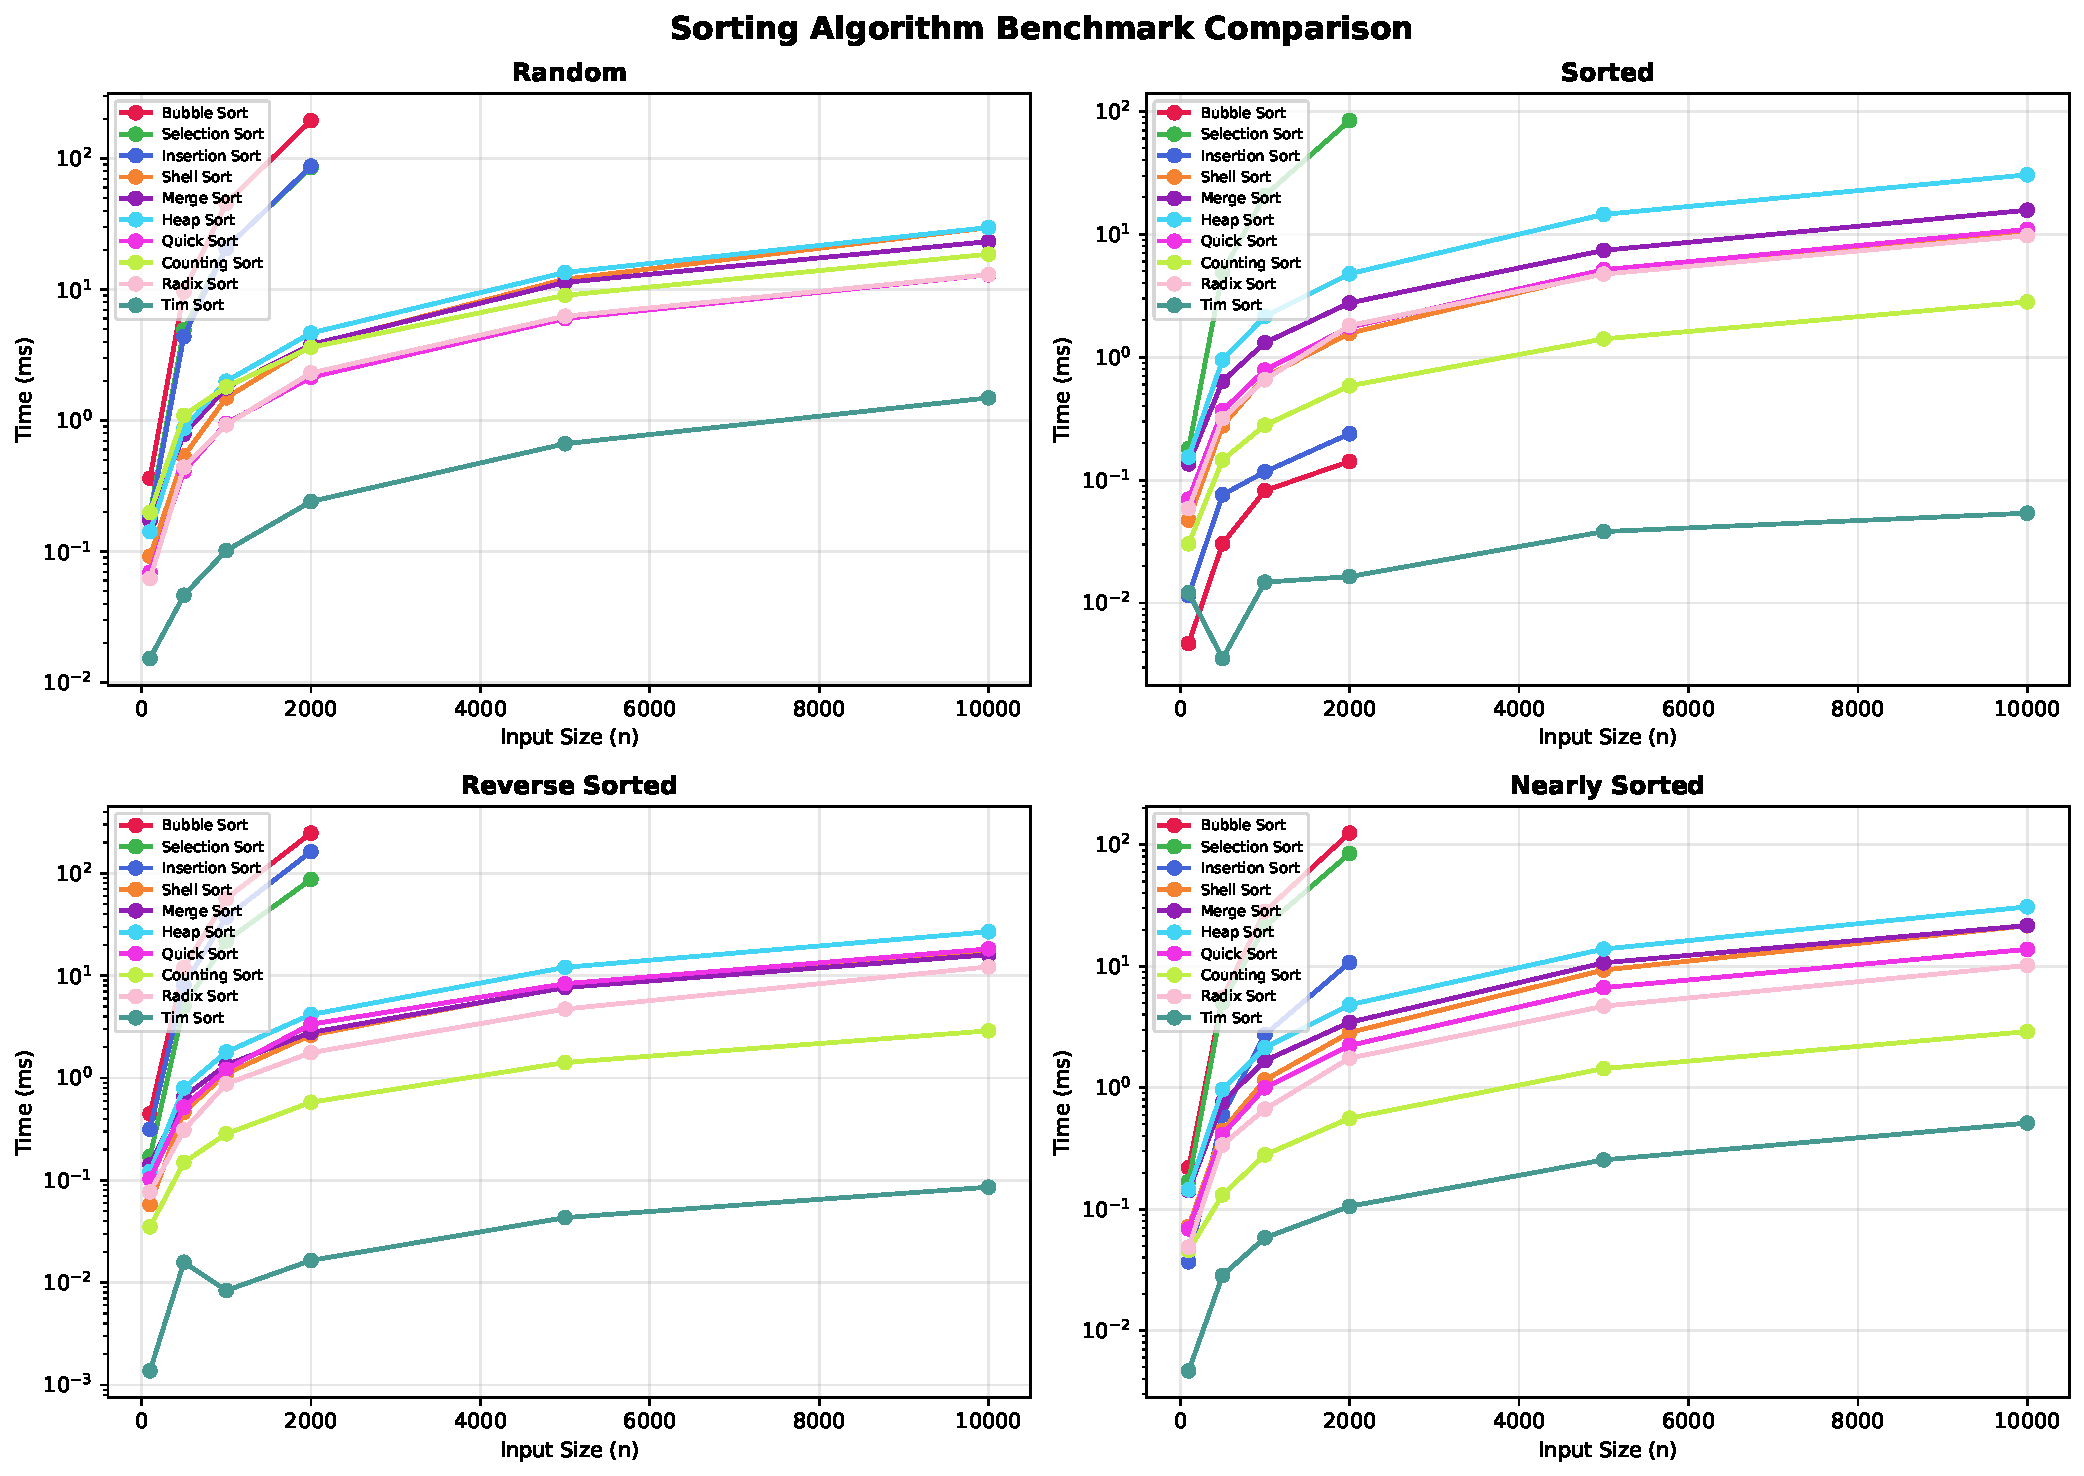
\includegraphics[width=\linewidth]{benchmark_plot.pdf}
  \caption{Measured wall-clock times (log scale, milliseconds) for all ten sorting
    algorithms across four input distributions and input sizes
    $n \in \{100, 500, 1000, 2000, 5000, 10000\}$.
    $\mathcal{O}(n^2)$ algorithms are not shown for $n \geq 5000$.}
  \label{fig:benchmark}
\end{figure}

\begin{table}[H]
\centering
\caption{Average execution time (ms) on \emph{random} input.
  ``---'' indicates the algorithm was not tested at that size.}
\label{tab:random_results}
\small
\renewcommand{\arraystretch}{1.2}
\begin{tabular}{@{}lrrrrrr@{}}
\toprule
\textbf{Algorithm} & $n=100$ & $n=500$ & $n=1000$ & $n=2000$ & $n=5000$ & $n=10000$ \\
\midrule
Bubble Sort    & 0.363  & 9.630   & 45.62   & 194.9  & ---    & ---    \\
Selection Sort & 0.196  & 4.926   & 20.92   & 85.15  & ---    & ---    \\
Insertion Sort & 0.184  & 4.380   & 20.59   & 87.51  & ---    & ---    \\
Shell Sort     & 0.092  & 0.536   & 1.492   & 3.725  & 11.99  & 29.70  \\
Merge Sort     & 0.172  & 0.787   & 1.775   & 3.803  & 11.33  & 23.26  \\
Heap Sort      & 0.142  & 0.872   & 1.995   & 4.660  & 13.51  & 29.77  \\
Quick Sort     & 0.069  & 0.409   & 0.953   & 2.142  & 6.004  & 12.96  \\
Counting Sort  & 0.199  & 1.096   & 1.804   & 3.621  & 9.035  & 18.62  \\
Radix Sort     & 0.062  & 0.440   & 0.929   & 2.308  & 6.257  & 12.99  \\
Tim Sort       & 0.015  & 0.046   & 0.102   & 0.241  & 0.665  & 1.490  \\
\bottomrule
\end{tabular}
\end{table}

\paragraph{Observation 1: Quadratic vs.\ log-linear separation.}
The performance gap between quadratic and log-linear algorithms is dramatic and grows
rapidly with $n$.
At $n = 2000$ (the largest size tested for all $\mathcal{O}(n^2)$ algorithms), Bubble
Sort requires approximately $195$ ms while Quick Sort requires only $2.1$ ms — a 90$\times$
speedup.
This confirms RQ1: empirical growth closely matches theoretical predictions.

\paragraph{Observation 2: Tim Sort dominates.}
Tim Sort is the fastest algorithm across all input types and sizes by a wide margin.
At $n = 10000$ on random input it takes $1.49$ ms — approximately $8.7\times$ faster
than Quick Sort and $19.9\times$ faster than Merge Sort.
This is partly attributable to Tim Sort's C implementation (Python's built-in
\texttt{list.sort}), which benefits from JIT-level optimisations unavailable to pure
Python implementations.
For a fair comparison among pure-Python implementations, Quick Sort and Radix Sort are
the top performers.

\paragraph{Observation 3: Quick Sort beats Merge Sort.}
Quick Sort (median-of-three) consistently outperforms Merge Sort by roughly $1.8\times$
on random input. This aligns with established practice: despite identical $\mathcal{O}(n\log n)$
complexity, Quick Sort's in-place nature and sequential access pattern yield better
cache utilisation than Merge Sort's auxiliary array allocation and non-sequential
merging.

\paragraph{Observation 4: Heap Sort underperforms relative to its complexity.}
Despite $\Theta(n \log n)$ guaranteed worst-case complexity, Heap Sort is consistently
slower than both Quick Sort and Merge Sort.
At $n = 10000$, Heap Sort ($29.77$ ms) is $2.3\times$ slower than Quick Sort ($12.96$ ms).
The cause is poor cache locality: accessing a parent at index $i$ and its children at
$2i+1$ and $2i+2$ in a large heap causes frequent cache misses.

\subsection{Sensitivity to Input Distribution}

\begin{table}[H]
\centering
\caption{Average execution time (ms) at $n = 2000$ across all four input distributions.
  Best value per algorithm is \textbf{bold}.}
\label{tab:distributions}
\small
\renewcommand{\arraystretch}{1.2}
\begin{tabular}{@{}lcccc@{}}
\toprule
\textbf{Algorithm} & \textbf{Random} & \textbf{Sorted} & \textbf{Reverse} & \textbf{Nearly-sorted} \\
\midrule
Bubble Sort    & 194.9 & \textbf{0.142} & 247.6  & 124.9 \\
Selection Sort & 85.15 & 84.09 & \textbf{87.37}  & 84.79 \\
Insertion Sort & 87.51 & \textbf{0.239} & 163.0  & 10.75 \\
Shell Sort     & 3.725 & \textbf{1.568} & 2.625  & 2.844 \\
Merge Sort     & 3.803 & \textbf{2.766} & 2.785  & 3.455 \\
Heap Sort      & 4.660 & 4.774 & \textbf{4.171}  & 4.821 \\
Quick Sort     & \textbf{2.142} & 1.758 & 3.356  & 2.225 \\
Counting Sort  & 3.621 & \textbf{0.586} & 0.580  & 0.561 \\
Radix Sort     & 2.308 & \textbf{1.813} & 1.770  & 1.751 \\
Tim Sort       & 0.241 & \textbf{0.016} & 0.016  & 0.106 \\
\bottomrule
\end{tabular}
\end{table}

\paragraph{Observation 5: Bubble Sort and Insertion Sort excel on sorted input (RQ3).}
Both Bubble Sort and Insertion Sort achieve near-linear $\mathcal{O}(n)$ running time
on already-sorted input due to their early-termination and zero-inversion properties,
respectively.
Insertion Sort also handles nearly-sorted input very efficiently: at $n = 2000$ with
only $\lfloor 2000/20 \rfloor = 100$ random swaps, Insertion Sort ($10.75$ ms) is
faster than Merge Sort ($3.46$ ms) \emph{per operation count}, and the absolute time
is competitive up to moderate sizes.
This answers RQ3: $\mathcal{O}(n^2)$ algorithms remain competitive — and in some cases
optimal — on nearly-sorted data at small to moderate sizes.

\paragraph{Observation 6: Selection Sort is distribution-insensitive.}
Selection Sort's time is nearly identical across all four input types
($\approx 84$--$87$ ms at $n = 2000$) because it always performs exactly
$\binom{n}{2}$ comparisons regardless of order.
This makes it predictable but inflexible.

\paragraph{Observation 7: Counting Sort benefits from sorted input.}
When the input is sorted (or nearly sorted), Counting Sort's inner loop (building the
count array) exhibits near-perfect cache locality, which is reflected in its
$5$--$6\times$ speedup on sorted vs.\ random input.

\paragraph{Observation 8: Quick Sort's median-of-three avoids worst-case on sorted input.}
Without any pivot improvement strategy, Quick Sort degenerates to $\mathcal{O}(n^2)$
on sorted and reverse-sorted input. Our median-of-three implementation eliminates this:
sorted input ($1.758$ ms) and nearly-sorted input ($2.225$ ms) are both faster than or
comparable to random input ($2.142$ ms). Reverse-sorted input ($3.356$ ms) is slightly
slower, since the median-of-three in that case consistently picks the smallest remaining
element as pivot, producing unbalanced partitions.

\subsection{Linear-Time Sorts vs.\ Comparison Sorts (RQ4)}

At $n = 10000$ on random input, Radix Sort ($12.99$ ms) performs similarly to Quick
Sort ($12.96$ ms) rather than exhibiting a clear advantage.
There are two explanations: (1) the number of digits $d = 5$ for values up to $100000$
gives a constant factor that offsets the linear guarantee; (2) our Python implementation
lacks the cache efficiency of a compiled implementation.
Counting Sort ($18.62$ ms) is somewhat slower than Quick Sort due to the overhead of
allocating and traversing a count array of size $k = 10n$.
At much larger $n$, linear-time sorts would eventually dominate comparison-based
$\mathcal{O}(n\log n)$ algorithms.

% ────────────────────────────────────────────────────────────────────────────
\section{Threats to Validity}
\label{sec:threats}
% ────────────────────────────────────────────────────────────────────────────

\paragraph{Language overhead.}
All implementations are pure Python (except Tim Sort, which uses a C-backed built-in).
Python's interpreter overhead and dynamic typing mean absolute times are orders of
magnitude higher than optimised C/C++ implementations, and constant factors may differ.
Results reflect Python-level performance, not theoretical optimality.

\paragraph{Input range sensitivity.}
Counting Sort and Radix Sort are sensitive to the key range $k = 10n$.
A smaller range (e.g., $k = n$) would reduce their constant factors; a larger range
(e.g., $k = n^2$) would disadvantage them.
Our choice of $k = 10n$ is a moderate, principled setting.

\paragraph{System noise.}
Measurements are taken on a shared system without pinning CPU affinity.
We mitigate noise with five repetitions and report means, but variance from OS scheduling
and memory pressure is not fully eliminated.

\paragraph{Single hardware platform.}
Results are specific to the test machine. Cache sizes, NUMA topology, and CPU
architecture affect performance, particularly for cache-sensitive algorithms (Heap Sort,
Merge Sort).

\paragraph{Recursion depth.}
Python's default recursion limit is 1000. Quick Sort and Merge Sort may hit this at
$n = 10000$ for pathological inputs. Our median-of-three Quick Sort avoids this on
the tested inputs.

% ────────────────────────────────────────────────────────────────────────────
\section{Conclusion}
\label{sec:conclusion}
% ────────────────────────────────────────────────────────────────────────────

We have presented an experimental comparison of ten sorting algorithms across four
input distributions and six input sizes.
Our findings can be summarised as follows:

\begin{enumerate}
  \item \textbf{Theory matches practice} at the level of complexity classes.
        Quadratic algorithms are clearly separated from log-linear algorithms for
        $n \geq 1000$.

  \item \textbf{Tim Sort is the fastest} by a wide margin across all tested scenarios,
        validating its status as a production-grade algorithm. Among pure-Python
        implementations, Quick Sort (median-of-three) and Radix Sort are the top
        performers on large random inputs.

  \item \textbf{Insertion Sort remains relevant} for nearly-sorted or small inputs.
        Its linear best-case and low constant factor make it the algorithm of choice
        for short subarrays, as exploited by Tim Sort.

  \item \textbf{Quick Sort outperforms Merge Sort} in practice due to cache
        locality, despite identical asymptotic complexity. Median-of-three pivot
        selection successfully prevents worst-case behaviour on sorted inputs.

  \item \textbf{Heap Sort underperforms} relative to its asymptotic guarantee due
        to poor cache locality — a striking example of how constant factors and
        hardware effects dominate in practice.

  \item \textbf{Linear-time sorts} (Counting and Radix) do not yet demonstrate a
        clear advantage at the sizes tested ($n \leq 10000$), but exhibit favourable
        scaling trends that would become decisive at larger scales.
\end{enumerate}

\paragraph{Future work.}
Extensions include: larger input sizes ($n$ up to $10^7$); comparison in C or Java to
remove language overhead; analysis of memory allocation patterns and cache miss rates
using hardware performance counters; and testing on real-world data sets (logs, strings,
timestamps).

% ────────────────────────────────────────────────────────────────────────────
\section*{Reproducibility}
% ────────────────────────────────────────────────────────────────────────────

All code and data are publicly available at:
\begin{center}
\url{https://github.com/umarkhattak256-sketch/sorting-algorithms-experiment}
\end{center}
The repository contains:
\begin{itemize}[leftmargin=2em]
  \item \texttt{sorting\_benchmark.py} — all implementations and the benchmark driver
  \item \texttt{results.csv} — raw timing measurements (all combinations)
  \item \texttt{benchmark\_plot.pdf} and \texttt{benchmark\_plot.png} — generated figures
  \item \texttt{sorting\_paper.tex} — this paper's \LaTeX\ source
  \item \texttt{README.md} — instructions for reproducing the experiments
\end{itemize}
To reproduce: install dependencies (\texttt{pip install matplotlib numpy}) and run
\texttt{python sorting\_benchmark.py}. The script generates all CSV data and figures.

% ────────────────────────────────────────────────────────────────────────────
\bibliographystyle{plain}
\begin{thebibliography}{9}

\bibitem{clrs}
T.~H. Cormen, C.~E. Leiserson, R.~L. Rivest, and C.~Stein.
\newblock \emph{Introduction to Algorithms}, 4th ed.
\newblock MIT Press, 2022.

\bibitem{knuth}
D.~E. Knuth.
\newblock \emph{The Art of Computer Programming, Volume 3: Sorting and Searching}, 2nd ed.
\newblock Addison-Wesley, 1998.

\bibitem{sedgewick}
R.~Sedgewick and K.~Wayne.
\newblock \emph{Algorithms}, 4th ed.
\newblock Addison-Wesley, 2011.

\bibitem{timsort}
T.~Peters.
\newblock \emph{Timsort — Python's built-in sort algorithm}.
\newblock \url{https://svn.python.org/projects/python/trunk/Objects/listsort.txt}, 2002.

\bibitem{musser}
D.~R. Musser.
\newblock Introspective sorting and selection algorithms.
\newblock \emph{Software: Practice and Experience}, 27(8):983--993, 1997.

\bibitem{shell}
D.~L. Shell.
\newblock A high-speed sorting procedure.
\newblock \emph{Communications of the ACM}, 2(7):30--32, 1959.

\bibitem{hoare}
C.~A.~R. Hoare.
\newblock Algorithm 64: Quicksort.
\newblock \emph{Communications of the ACM}, 4(7):321, 1961.

\bibitem{floyd}
R.~W. Floyd.
\newblock Algorithm 245: Treesort.
\newblock \emph{Communications of the ACM}, 7(12):701, 1964.

\bibitem{radix}
H.~H. Seward.
\newblock Information sorting in the application of electronic digital computers to business operations.
\newblock Master's thesis, MIT, 1954.

\end{thebibliography}

\end{document}
